% !TEX TS-program = pdflatex
% !TEX encoding = UTF-8 Unicode

% This is a simple template for a LaTeX document using the "article" class.
% See "book", "report", "letter" for other types of document.

\documentclass[11pt]{article} % use larger type; default would be 10pt

%\usepackage[utf8]{inputenc} % set input encoding (not needed with XeLaTeX)


%%% Examples of Article customizations
% These packages are optional, depending whether you want the features they provide.
% See the LaTeX Companion or other references for full information.

%%% PAGE DIMENSIONS
\usepackage{geometry} % to change the page dimensions
\geometry{a4paper} % or letterpaper (US) or a5paper or....
\geometry{margin=1in} % for example, change the margins to 2 inches all round
% \geometry{landscape} % set up the page for landscape
%   read geometry.pdf for detailed page layout information

\usepackage{graphicx} 
% \usepackage[parfill]{parskip} % Activate to begin paragraphs with an empty line rather than an indent

%%% PACKAGES
%\usepackage{booktabs} % for much better looking tables
\usepackage{array} % for better arrays (eg matrices) in maths
%\usepackage{paralist} % very flexible & customisable lists (eg. enumerate/itemize, etc.)
\usepackage{verbatim} % adds environment for commenting out blocks of text & for better verbatim
%\usepackage{subfig} % make it possible to include more than one captioned figure/table in a single float
% These packages are all incorporated in the memoir class to one degree or another...

%%% HEADERS & FOOTERS
\usepackage{fancyhdr} % This should be set AFTER setting up the page geometry
\pagestyle{fancy} % options: empty , plain , fancy
\renewcommand{\headrulewidth}{0pt} % customise the layout...
\lhead{}\chead{}\rhead{}
\lfoot{}\cfoot{\thepage}\rfoot{}

%%% SECTION TITLE APPEARANCE
%\usepackage{sectsty}
%\allsectionsfont{\sffamily\mdseries\upshape} % (See the fntguide.pdf for font help)
% (This matches ConTeXt defaults)

%%% ToC (table of contents) APPEARANCE
%\usepackage[nottoc,notlof,notlot]{tocbibind} % Put the bibliography in the ToC
%\usepackage[titles,subfigure]{tocloft} % Alter the style of the Table of Contents
%\renewcommand{\cftsecfont}{\rmfamily\mdseries\upshape}
%\renewcommand{\cftsecpagefont}{\rmfamily\mdseries\upshape} % No bold!

%\usepackage[T1]{fontenc}
\usepackage[latin9]{inputenc}
%\usepackage[active]{srcltx}
\usepackage{setspace}
\doublespacing
\usepackage[english]{babel}

\begin{document}

\title{Connectivity Analysis of Metagenomic Data}
\author{ACH, JP, RCK, RM, JJ, JMT, CTB}
\maketitle
\section{Introduction}

Given the rapid decrease in the costs of sequencing, we can now achieve the sequencing depth necessary to study even the most complex environments \cite{Hess:2011p686,Qin:2010p189}.  Currently, the major challenges in metagenomic studies are the continuously increasing number of sequencing reads and the lack of effective strategies to annotate and predict gene functions from these short reads \cite{Hoff:2009p913,Kunin:2008p16,Noguchi:2006p968,Zhang:2012p959}.  De novo metagenomic assembly of these reads offers several solutions.  Firstly, assembly significantly reduces the data size by collapsing numerous short reads into relatively fewer contigs, providing longer sequences containing multiple genes and operons \cite{Miller:2010p226,Pop:2009p798}.  Because it does not rely on the availability of reference genomes, de novo metagenomic assembly also produces novel contigs and create opportunities for further analysis, such as comparisons of novel sequences within and between metagenomes \cite{Li:2009p707,Schloss:2008p2} or annotations of novel genomes \cite{Hess:2011p686}.

The general strategy for metagenomic assembly has been to use de novo \emph{genome} assemblers \cite{Hess:2011p686,Qin:2010p189}, particularly those targeting the assembly of short read sequences such as de Bruijn graph assemblers (reviewed in \cite{Miller:2010p226,Pop:2009p798}). These single genome assemblies are complicated by repetitive sequences, sequencing errors, and sequencing biases, and within the de Bruijn assembly graph, these elements increase graph complexity. For single genome assembly, relatively low rates of polymorphisms and sequencing errors are assumed to enable read coverage to determine the correct assembly path through the graph (cite some assemblers here).  For metagenomic assembly, these assumptions do not hold true, and coverage-based resolution of the metagenomic assembly graph is confounded by the presence of multiple organisms which may both be closely related to each other and sampled at unequal depths \cite{Peng:2011p898}.  De novo metagenomic assembly is further complicated by the presence of sequencing errors and/or artifacts which current assemblers cannot distinguish from variable-coverage genomic sequences \cite{Peng:2011p898,Venter:2004p727}.  The presence of such sequencing biases is known in Illumina sequences \cite{Harismendy:2009p228,Hoffmann:2009p1027,Nakamura:2011p741}, but their effects on assembly graph properties and thus resulting assemblies is largely unstudied. 
  
The significant depth of sequencing which is needed to study complex environments presents specific challenges to metagenomic de novo assembly.  Assemblers must not only be able to scale to these larger datasets but also be able to deal with the increasing amounts of sequencing errors and biases that accompany real biological sequences.   A better understanding of the assembly graph and the effects of sequencing artifacts for these complex metagenomic datasets is critical to improving de novo metagenomic sequence assembly.  In this study, we analyze the graph structures and connectivity of several metagenomic datasets and present our findings of highly-connecting sequences which are observed in all metagenomes we studied.  We suggest that a significant portion of these sequences are sequencing artifacts and examine the effects of their removal on metagenomic assembly.

\section{Results and Discussion}
\subsection{Connectivity analysis of metagenome datasets}

We selected datasets from three diverse, medium to high complexity metagenomes from the human gut \cite{Qin:2010p189}, cow rumen \cite{Hess:2011p686}, and agricultural soil (unpublished). For comparison, we also included one simulated metagenome (error-free) of a high complexity, high coverage (\textasciitilde{}10x) microbial community \cite{Pignatelli:2011p742}. To study the effects of increased sequencing, we also included two additional subsets of the agricultural soil metagenome containing 50 million and 100 million reads each. 

The connectivity of reads within datasets were evaluated within a de Bruijn graph representation (see Methods). For all datasets, both real and simulated, we found that the assembly graph was dominated by a single, highly connected "lump'' of sequencing reads (Figure 1, Table 1). In the human gut dataset, over 75\% of the sequencing reads were associated with this lump. Likewise, from the rumen and 500 million read agricultural dataset, a total of 21\% and 39\% of all reads, respectively, were observed to be highly connected. Within the simulated dataset, the lump was smaller in size encompassing approximately 5\% of the reads. Interestingly, for the three soil datasets, the increase in the size of the lump was not proportional to increases in the amount of sequencing (Figure 1, Table 1).  As the number of reads increased by 2-fold and 5-fold, the size of the lump increased by 5-fold and 14-fold, respectively. This supra-linear increase of lump size relative to the increase of number of reads suggests that the connectivity of reads within a lump increases more rapidly than the contents of the lump.  

There are multiple causes of the observed highly-connected lump within metagenomic datasets.  In general, the lump is the result of overlapping sequences from metagenomic.  These sequences could have originated from genes which are conserved across multiple genomes (i.e. 16S rRNA, ITS regions).  However, the size of the lump and the effects of increasing dataset size on this size indicate that non-biological artifacts are likely involved in creating the lump.  An alternative explanation is that the lump is the result of the presence of sequencing biases causing high-connectivity between metagenomic reads.  In this case, we would expect a rapid accumulation of sequences into the lump as more sequencing is added, a phenomenon we call "preferential attachment".   Highly connecting "X" sequences in a lump would recruit a number of connecting "Y" reads into the lump.  As more sequences are added, these "Y" reads, which do not necessarily have to be highly-connective, would recruit more "Z" reads into the lump resulting in increasingly larger lump size.  This effect of "preferential attachment" is observed in the increasing size of the soil metagenomes causing larger lumps. 

To further explore this hypothesis and better understand the connectivity of metagenomic reads, we measured the local graph density of reads within the de Bruijn assembly graph. The local graph density is defined here as the number of k-mers found within a distance of N divided by N.  In the case of a linear sequence, the local graph density would be 2, and additional branches or repeats would increase this value. For each of the studied datasets, we compared the local graph densities of the k-mers (nodes) within the de Bruijn assembly graph.  For the human gut, rumen, and corn metagenome (500 million reads), over 90\% of the nodes had an average graph density greater than 20 (Need to rerun on metahit).  In comparison, the density of the assembly graphs of a mixture of microbial genomes (112 genomes) and the complementary simulated dataset both had fewer than 2\% of the nodes with an average graph density greater than 20.  

The combination of the presence of a large, highly-connected lump and high local graph densities in environmental metagenome assembly graphs suggest the presence of substantial spurious connectivity within these metagenomic sequences.  Systematic biases in base calling would create such connectivity and can often be observed as position-specific within sequencing reads.  We proceeded to look for non-uniform properties of highly-connecting sequences within sequencing reads.

\begin{figure}
\center{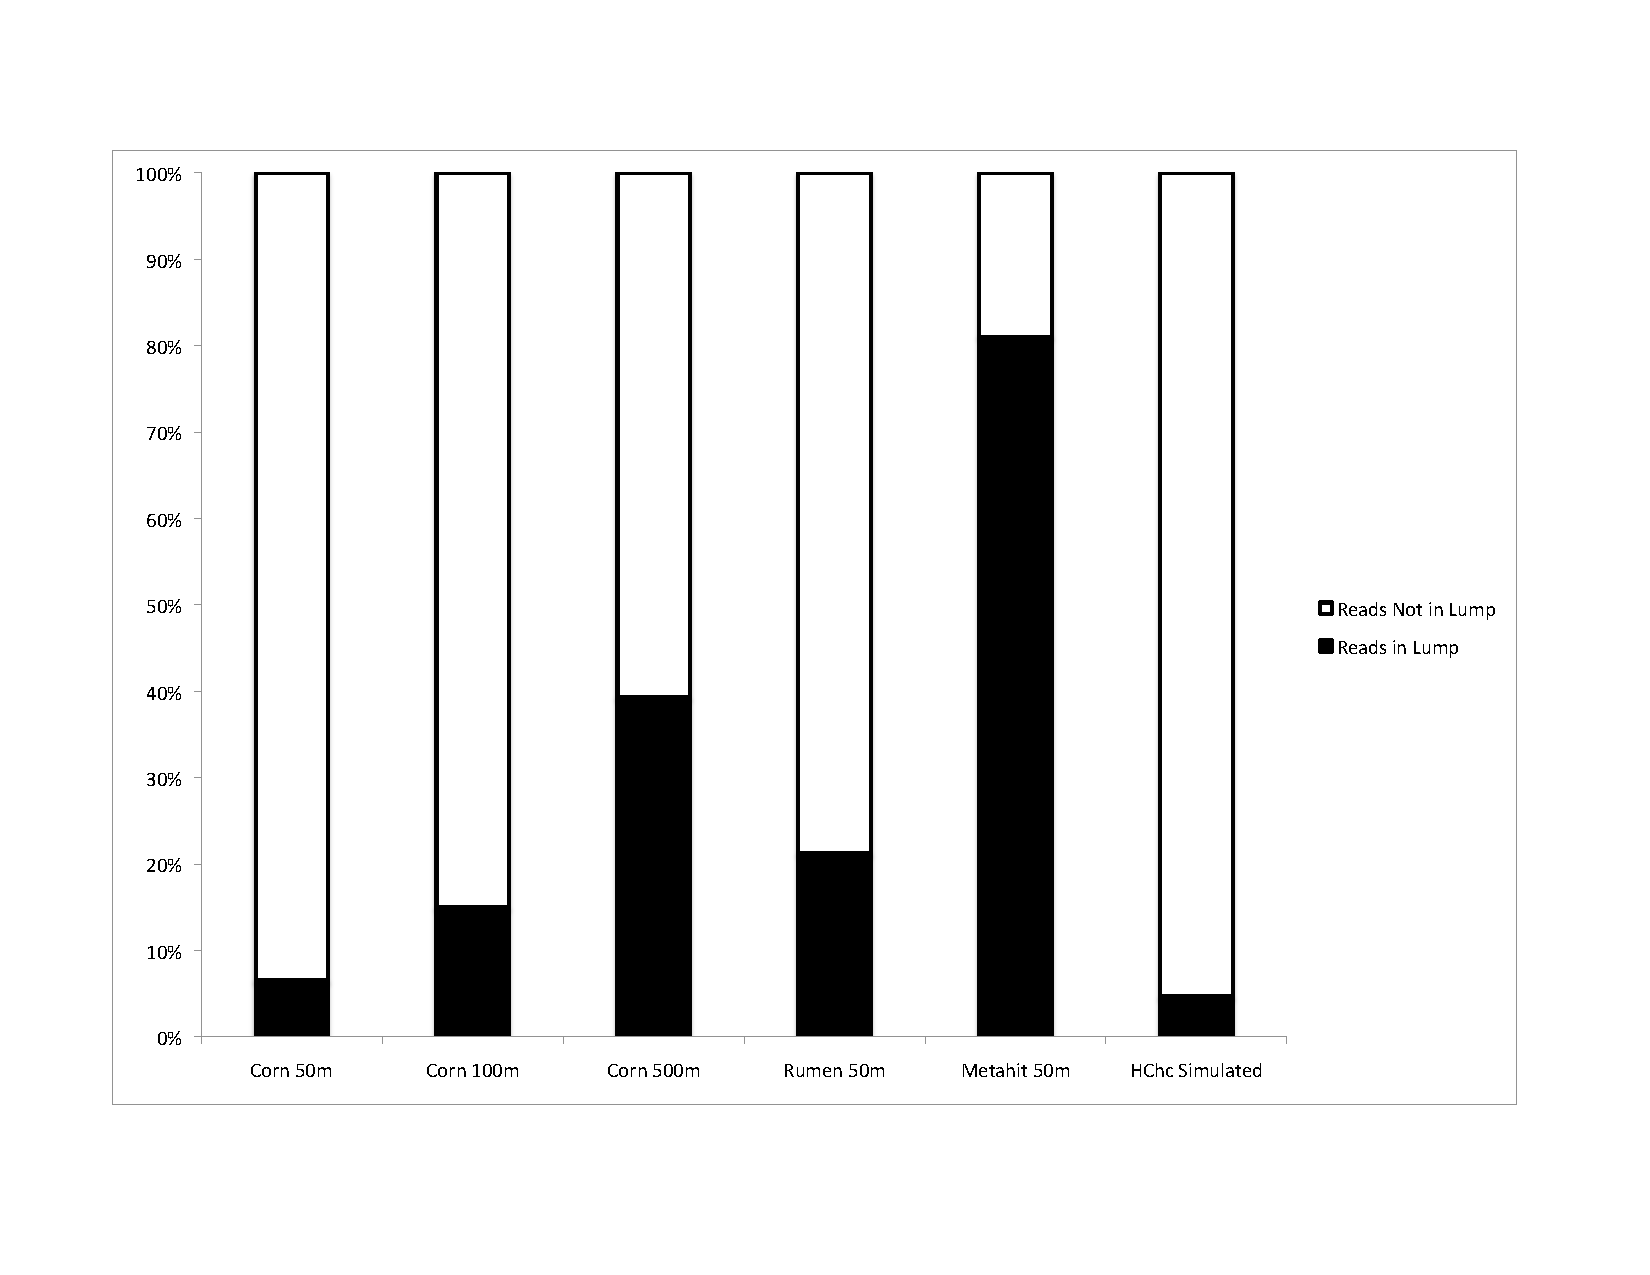
\includegraphics[width=5in]{./figures/lumps.pdf}}
\caption{The largest proportion of total reads which are connected to each other within a "lump".}
\end{figure}

\begin{table}
\center{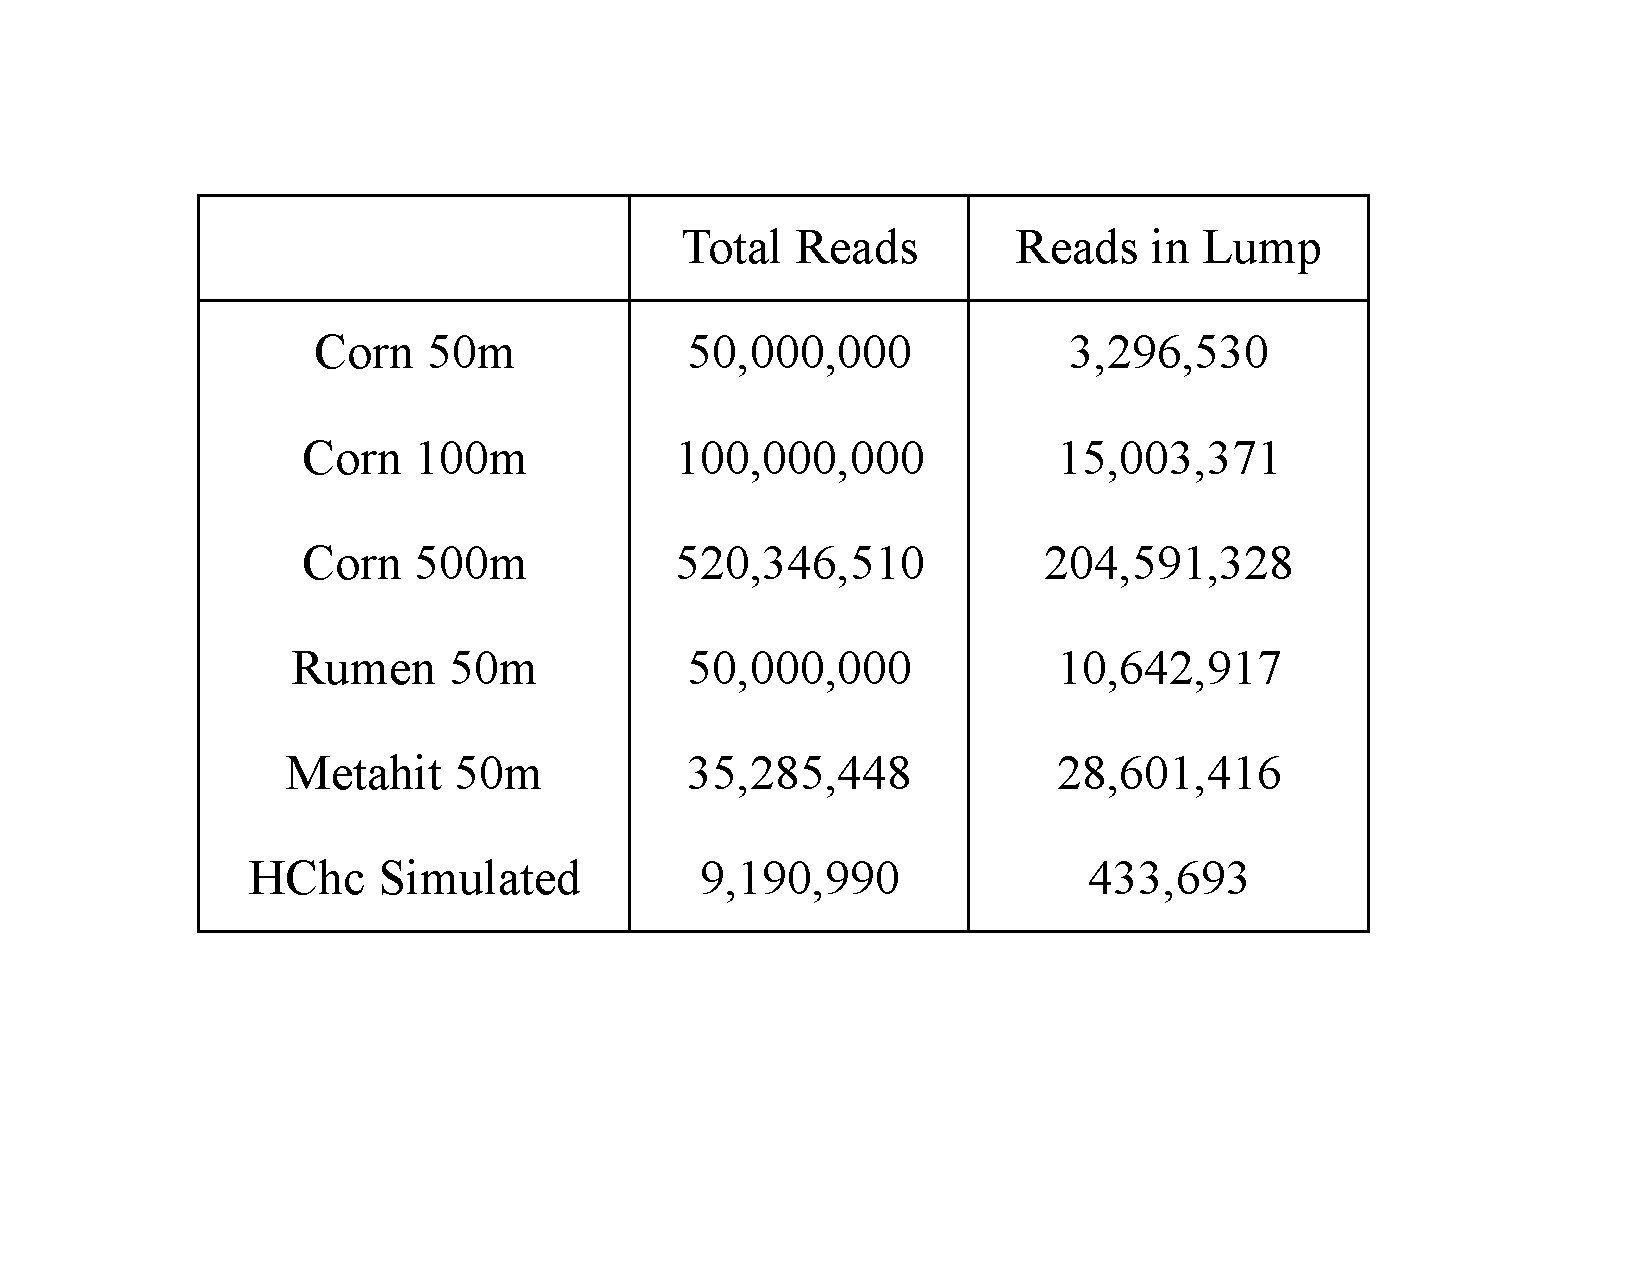
\includegraphics[width=5in]{./figures/lump_table.pdf}}
\caption{Total number of reads in each dataset and corresponding largest connected subset lump}
\end{table}


\subsection{Properties of highly connected sequences in sequencing reads}

We used a systematic traversal algorithm to identify the highly-connecting k-mers within the de Bruijn graph of each metagenome's lump (see Methods).  These sequences were flagged as probable causes to "knots" in our highly-connected lump and likely causes of the lump itself.  To study position-specific effects of these sequences, the location of knot-causing sequences (k-mers) were identified in originating sequencing reads.   
	As shotgun sequencing fragments are randomly generated and sequenced, one does not expect any position specific bias of sequences within reads.  This is observed in the simulated dataset where we observe no position-specific effects of the knot-causing sequences.  Cumulatively, the fraction of these sequences normalized to total sequences in the lump is relatively stable at all positions in the read (Figure 2).  Contrastingly, in metagenomic lumps regardless of origin, we found that the position of knot-causing sequences within the read were biased towards one end of the read.  In the soil metagenomes, a large fraction of knot-causing sequences were found at the 3' end of the read.  In the human gut and rumen reads, smaller fractions of these sequences were located at the 3' end of the reads.  Overall, the observed non-uniform position specific bias of the knot-causing sequences within metagenomes demonstrates the presence of systematic biases in base calling. 
	The observed differences in the direction of position specific biases within the different metagenomes was unexpected. A possible explanation for the observed differences may be actual differences in sequencing biases between the creation of different sequencing libraries (i.e. changes in Illumina chemistry, etc).  Alternatively, the previously described phenomenon of preferential attachment may be causing the recruitment of specific reads which are correlated to the coverage of the metagenome.  The human gut and rumen environments are much less complex than the soil and have higher sequencing coverage.  In the case of the human gut and rumen metagenomes, It is plausible that more overlapping high-coverage reads were recruited into the lump by preferential attachment.  These reads would increase the total number of non-knot-causing sequences and dilute the signal of knot-causing sequences within these metagenomes.  This explanation is also supported by the trends observed with increasing dataset size of the soil metagenomes as the fraction of knot-causing 3' position-specific bias decreased with increasing sequencing coverage.

\begin{figure}
\center{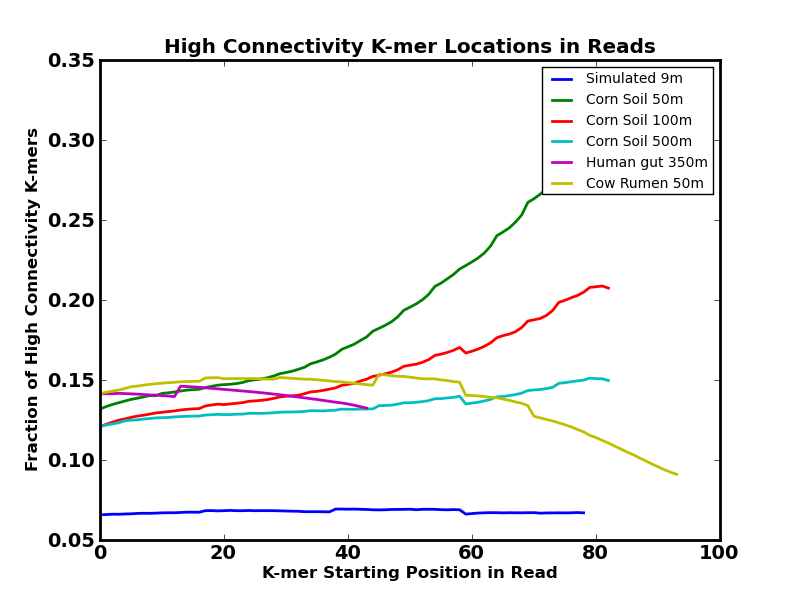
\includegraphics[width=5in]{./figures/pos-spec-bias.png}}
\caption{Position specific biases are observed in metagenomes but not in simulated data.  For each position, the ratio of total number of knot-causing 32-mers and total number of 32-mers for all reads was determined.}
\end{figure}

\subsection{Effects of removing highly connected sequences in assemblies }

Next, we evaluated the effects of the knot-causing sequences on the assemblies of each metagenome (Table 2).   We compared the set of shared constituent k-mers between original and knot-filtered assemblies as well as several standard assembly metrics (total number of contigs, maximum contig size, and number of assembled base pairs). For the simulated dataset, removal of knot-causing sequences resulted in an assembly which contained 90\% of the same constituent 32-mers as the original assembly.  The simulated original and knot-filtered assemblies also shared similar totals of assembled contigs (greater than 500 bp), number of assembled base pairs, and maximum contig size. In real metagenomes (human gut, rumen, and soil), original and knot-filtered assemblies had similar numbers of contigs but had significant differences in the number of base pairs and maximum contig sizes within the assemblies.  The Velvet-assembled rumen knot-filtered assembly resulted in approximately 1,000 less contigs, over 1 million more assembled base pairs, and a 2-fold increase in maximum contig size with the removal of nearly 8\% of the total unique k-mers.  In general, most of the unfiltered and knot-filtered assemblies were similar, sharing greater than 70\% of constituent k-mers (with the exception of the soil metagenome with 100 million reads).    

\begin{table}
\center{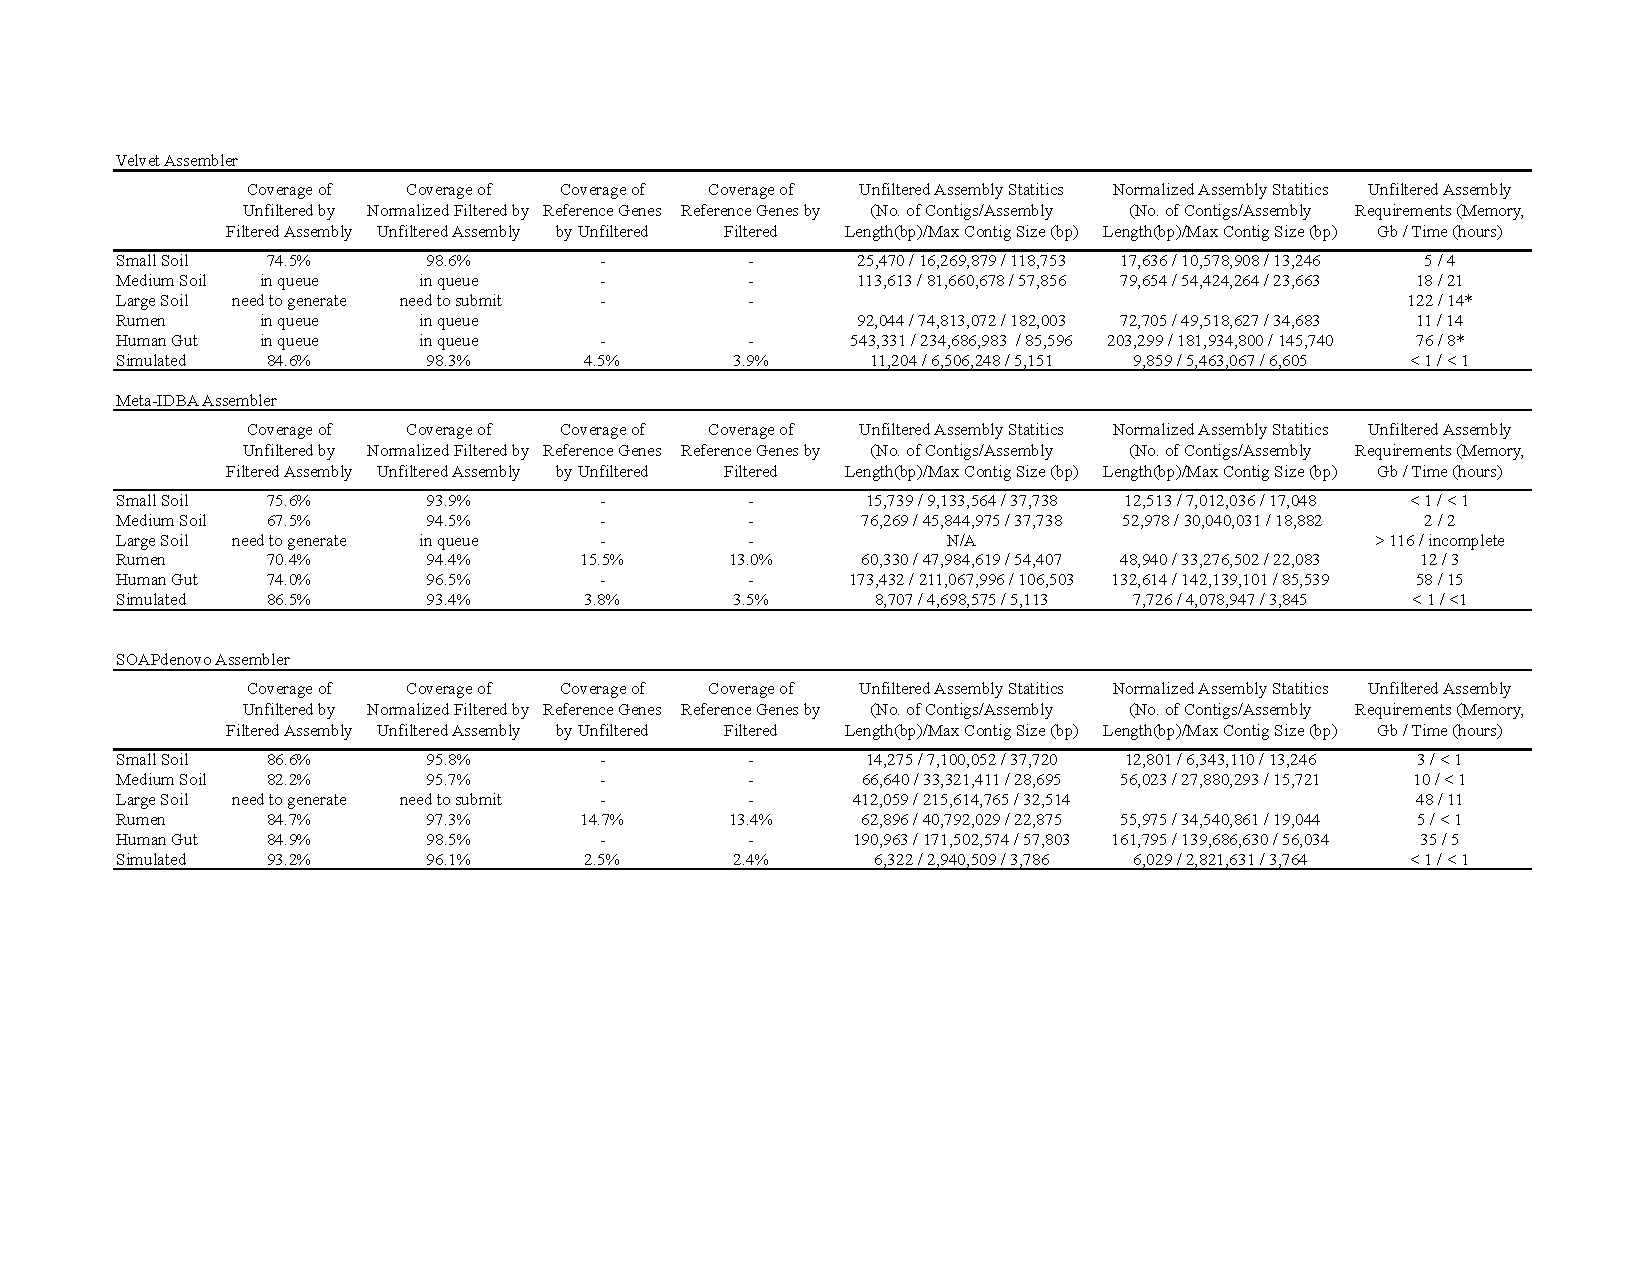
\includegraphics[width=5in]{./figures/assembly_comparison.pdf}}
\caption{Comparison of assembly (Velvet) of metagenome reads in lump with and without removal of knot-causing sequences.  Percent similarity of assemblies was determined by determining overlap of constituent 32-mers between assemblies.}
\end{table}

\subsection{Effects of highly connected sequences in unfiltered assemblies}
As the removal of knot-causing sequences did not greatly change the assemblies, we expected that the knot-causing sequences were not highly present in assembled contigs.  We compared the presence of the knot-causing sequences in the original reads to the assembled contigs.  We found that in all the datasets, sequencing reads were significantly more enriched for knot-causing sequences over the final assembled contigs. In the simulated dataset, nearly 7 times more knot-causing sequences were present in reads than in assembled contigs. In metagenomic reads, these sequences were 1.8 to 6.5 times more prevalent in reads than assembled contigs (Table 3).  These results suggest that highly-connecting sequences, regardless of biological (as in the simulated dataset) or artifactual origin, are not effectively incorporated into assembly (observed in both Velvet and Abyss).  Thus, removal of these knot-causing sequences should minimally affect assemblies.  

We were subsequently interested in quantifying the contribution of knot-containing contigs to observed unfiltered and knot-filtered assembly differences.  To crudely estimate the effects of the knot-causing sequences incorporated into unfiltered contigs, we counted the total number of k-mers in contigs which contained knot-causing sequences and compared this to the total number of unique constituent k-mers which differed between unfiltered and filtered assemblies.  The knot-causing sequences of contigs in the rumen and soil metagenomes accounted for less than  3\% of the estimated difference in assemblies.  In the human gut assemblies, knot-causing sequences accounted for 22\% of the estimated difference between assemblies.  As these estimates are based on k-mer content differences of the total length of knot-containing contigs, they over-estimate the contribution of knot-causing sequences to unfiltered and knot-filtered assembly differences.   Overall, these results further support that removal of knot-causing sequences does not significantly affect the resulting assembly.


\begin{table}
\center{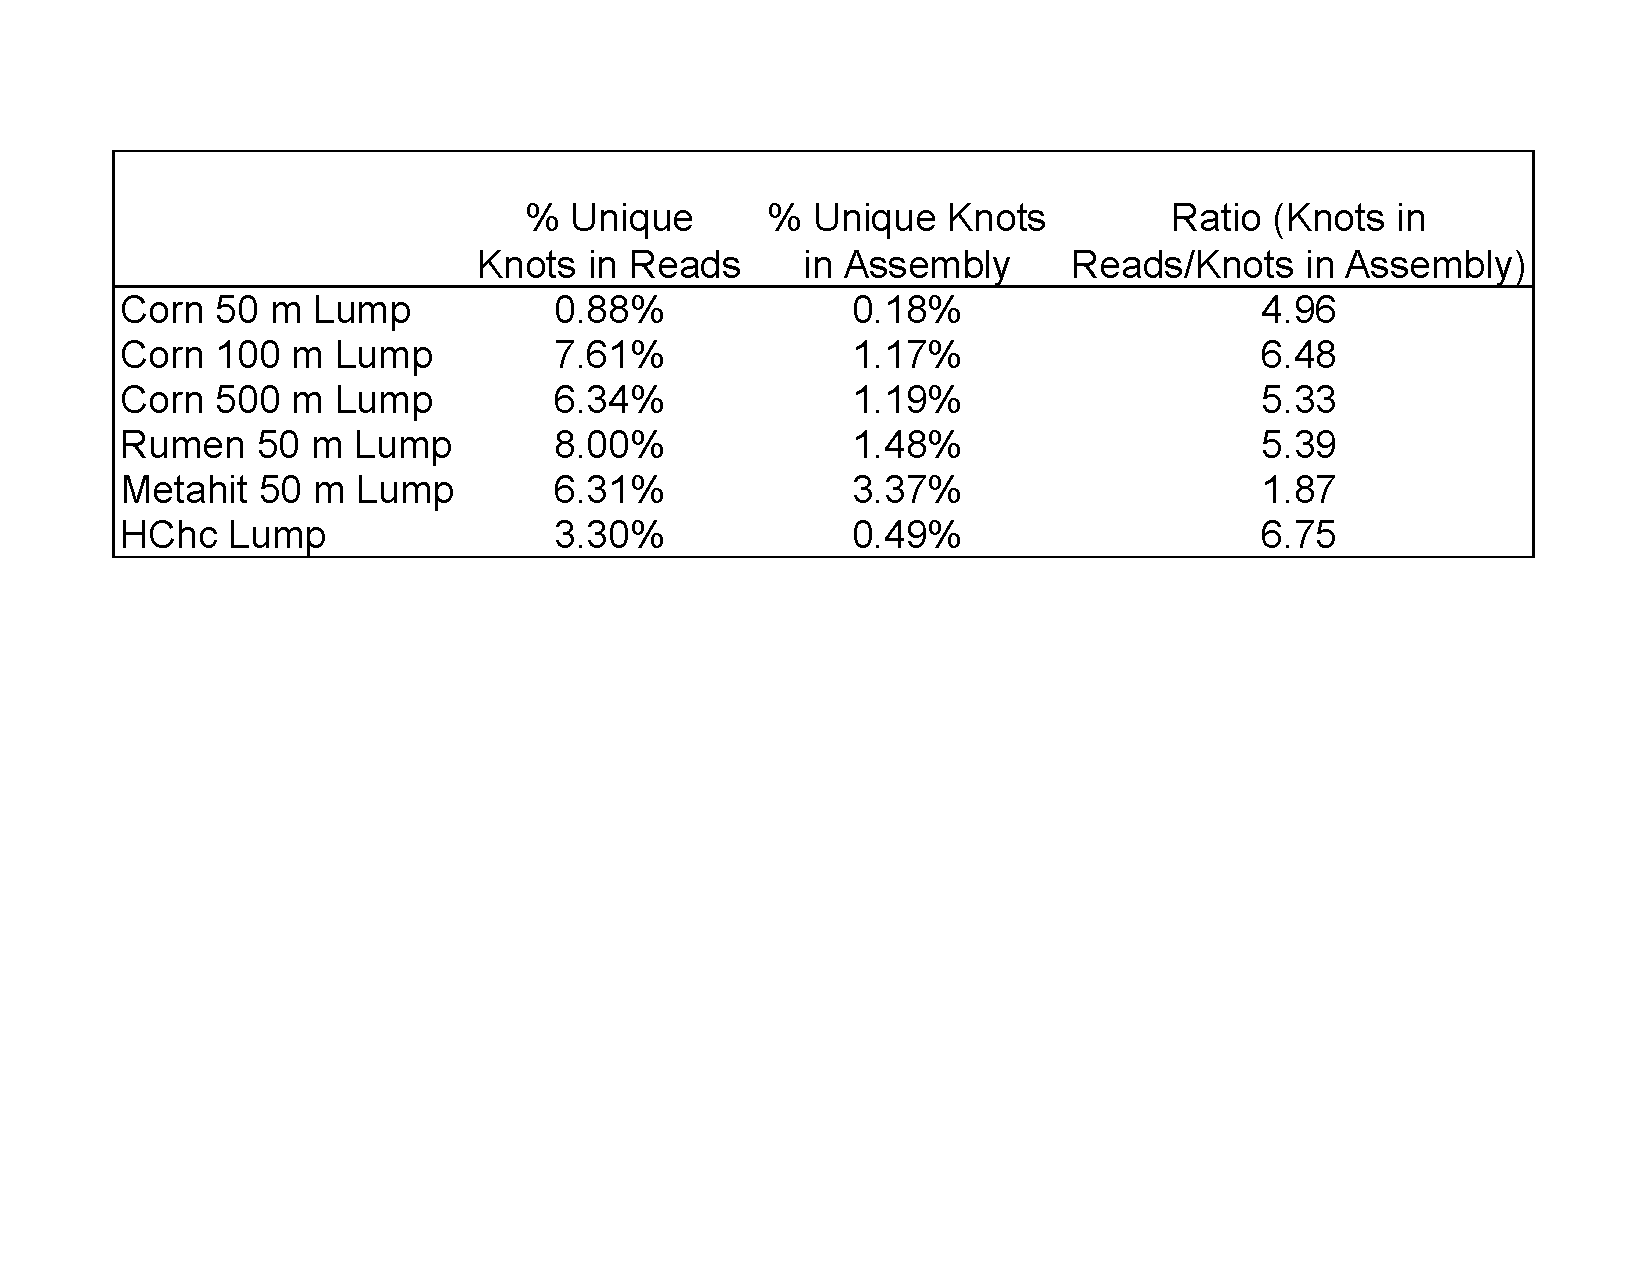
\includegraphics[width=5in]{./figures/knot_enrichment_in_reads.pdf}}
\caption{Lack of knot-causing sequences in assembled contigs in all metagenomes and simulated data.}
\end{table}


\subsection{Properties of highly connected sequences in assembled contigs}

Given that the knot-causing sequences are not significantly being incorporated into the final assembly, we were interested in the location of these sequences in the assembly.  We examined the position of the knot-causing sequences within assembled contigs and observed that they were disproportionately being placed on the ends of the contigs (Figure 3).  The presence of these sequences on the ends of contigs would contribute to observed differences in unfiltered and knot-filtered assemblies.  A specific contig cutoff length was used to filter contigs for assembly accuracy.  In this study, we included only contigs greater than 500 bp.  If knot-causing sequences are located on the ends of contigs, their removal would affect the total length of the contig and consequently its consideration in the final assembly.  For example, a 32-bp knot-causing sequence fragment on the end of a 499 bp assembled contig would result in a 531 bp contig in an unfiltered assembly.  When comparing constituent k-mers of these two assemblies, the k-mers contributed by this contig (length=499 bp) would be entirely lost in the knot-filtered assembly if the contig cutoff length were 500 bp.  The loss of such contigs and their constitutive k-mers would contribute to the differences observed between unfiltered and knot-filtered assemblies.  Further differences would also occur from trimming the sequences of the original reads and thus changing their connectivity in the assembly graph, but these changes are more difficult to measure.  

\begin{figure}
\center{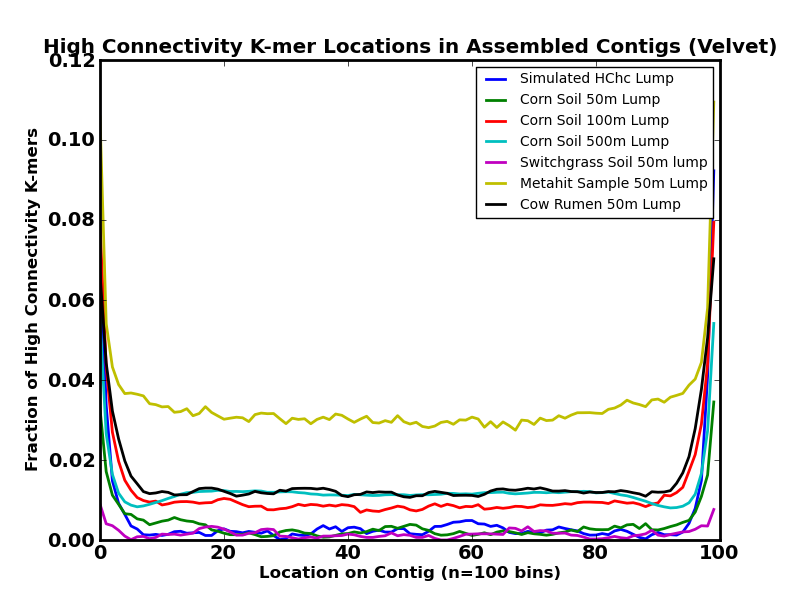
\includegraphics[width=5in]{./figures/pos-spec-bias-contigs.png}}
\caption{Knot-causing sequences are disproportionately being placed at the ends of assembled contigs.  Each contig was into 100 equal-length bins.  For all contigs, the ratio of total number of knot-causing 32-mers and total number of total 32-mers within each bin was determined.}
\end{figure}


\subsection{Properties of highly connected sequences in assembled contigs}
Since knot-causing sequences are preferentially being assembled at the ends of contigs, we hypothesized that many of these sequences may be erroneously assembled.   Evaluating the accuracy of metagenomic assemblies is challenging because we have limited knowledge of the original microbial composition.  Ideally, known genomes from the studied system could be used to partially evaluate assemblies.  Given the lack of reference genomes for the studied metagenomes, we used an alternative method to evaluate assemblies.  Contigs were evaluated by the content of predicted protein coding genes, or open reading frames (ORFs).  Since we hypothesized that knot-causing sequences are being misassembled, we expect these sequences to be located at the "edge" of an ORF, thus truncating the protein coding region, or outside of an ORF.  We considered an ORF "edge" to be the sequences partially contained inside an identified ORF and partially extended beyond the ORF.    
	Within all datasets, we observed a significant enrichment of knot-causing sequences at the edges of ORFs. In the metagenomes, we observed between a 2x and 4x enrichment of these sequences at ORF edges (Figure 4).  To come:  Insert something here about checking assembly against reference genomes....(waiting for metahit results as it contains the largest reference set) 
	Interestingly, in the simulated dataset, we observed a 5x enrichment of knot-containing sequences at ORF edges.  Among the contigs which contained knot-causing sequences enriched at ORF edges, only 2 of 85 contigs contained mismatches to the best alignment of originating genomes suggesting accurate assembly of these sequences.  We then considered the effects of removing knot-causing sequences on the accuracy of gene annotation by comparing the alignment lengths of ORFs from the original and knot-filtered assemblies to protein references.  We found that the large majority of alignment lengths did not change (83\%, 1229 ORFs), some of the alignment lengths were worsened by filtering (10\%, 151 ORFs), and some of the alignment lengths were improved by filtering (7\%, 105 ORFs).  In other words, removal of the knot-containing sequences had small effects on overall assembly of the simulated dataset.  
	
	
	

\begin{figure}
\center{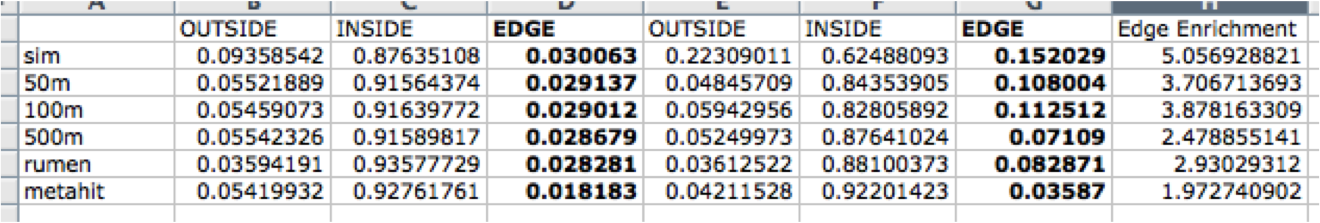
\includegraphics[width=5in]{./figures/temp-orfs.png}}
\caption{I'll make this better later.}
\end{figure}

\section{Conclusions}

Short-read sequencing technologies, such as the Illumina platform, are creating unprecedented opportunities to deeply study complex environments.  Sequence assembly and annotation, rather than sequence generation, are now the major limitations for metagenomic studies of environmental systems.  Coincidently, an understanding of the nature of metagenomic sequences is of paramount importance to building specific tools for their analysis.  In this study, we have demonstrated the presence of sequencing biases contributing to artificial sequence connectivity and suggest that removing these sequences does not significantly change the resulting assemblies. Our analysis also shows that the number of highly-connecting sequences increases significantly with increasing sequencing datasets.  Thus, these artifactual sequences not only contribute to erroneous assemblies and gene annotations but also interfere with the ability to break apart the assembly graph which is a potential solution for scaling assembly for complex metagenomes. New approaches for de novo metagenomic assembly apply the properties of the assembly graph structure to resolve confounding assembly paths. These assemblers decompose the de Bruijn graph and subsequently perform iterative assemblies of isolated components \cite{Peng:2011p898} (Namike 2011 unpublished).  A better understanding of the effects of sequencing biases on these approaches is necessary to effectively use them to generate accurate assemblies.  

	Critical analysis of sequencing biases and errors in metagenomic datasets would extend beyond de novo metagenome assembly.  For example, very little is known about the true diversity in environments and the depth of sequencing needed to obtain appropriate coverage of an environment.  Available metagenomic datasets are often used to estimate these parameters, and without accounting for sequencing errors and biases, these estimates will be largely inaccurate.  The ability to make conclusions from deep metagenomic sequencing depends on efforts and tools to understand the data itself.  Our efforts highlight the usage of connectivity analysis within an assembly graph representation to identify and evaluate potential sequencing artifacts.  Future efforts to better understand the origin of these sequencing artifacts and their effects on other metagenomic analysis would be valuable.  For assistance, we provide the sequencing datasets, knot-causing sequences, and unfiltered and filtered assemblies used in this study at lyorn:/scratch/adina/artifacts-datasets.
	

Do we want to discuss this?  I vote no.
The recently published metagenomes of the human gut (Qin et al, 2011, enterotype) and cow rumen (Hess et al., 2011) highlight the successful combination of high coverage Illumina sequencing with de novo metagenome assembly to identify prevalent ecosystem genes.  In both these studies, assembly of short sequencing reads was limited by the metagenome complexity, which is directly affects assembly memory requirements (>512 Gb for both metahit and cow rumen metagenomes).  In order to complete assembly of these metagenomes, low abundant sequences were initially removed to decrease the metagenome complexity and size.  For more complex environments, such as the soil, equivalent filtering strategies would result in the elimination of a significant majority of the sequencing library.   

\section{Methods}

\subsection{Metagenomic datasets}

All datasets, with the exception of the agricultural soil metagenome, were from
previously published datasets. Rumen-associated sequences (Illumina)
were randomly selected from the rumen metagenome available at ftp://ftp.jgi-psf.org/pub/rnd2/Cow\_Rumen. Human-gut associated sequences (Illumina) of sample MH0086 were obtained from ftp://public.genomics.org.cn/BGI/gutmeta/Raw\_Reads. This sample
was selected because of the relatively high number of reads reported
as assembled (53.7\%) (Qin et al, 2010). The agricultural
soil metagenome was from the sequencing (Illumina) of Iowa corn soil and is currently unpublished. All reads used in this study were quality-trimmed for Illumina's read segment quality control indicator, where a quality score of 2 indicates that all subsequent
regions of the sequence should not be used. After quality-trimming,
only reads with lengths greater than 30 bp were retained. All quality
trimmed reads used in this study are available at X. After quality-trimming,
the rumen and human gut datasets contained a total of 50 and
35 million reads, respectively. The agricultural soil dataset contained
a total of 520 million reads from which 50 and 100 million reads were
randomly sampled as subsets. The simulated high complexity, high coverage
dataset was previously published (Pignatelli, 2011). It was randomly
selected from a set of 112 complete genomes and contained a total
of 9 million reads.


\subsection{Lightweight, compressible de Bruijn graph representation}

We used a lightweight probabilistic de Bruijn graph representation
to explore k-mer connectivity of the assembly graph (cite paper?).
The de Bruijn graph stores k-mer nodes in Bloom filters and keeps
edges between nodes implicitly, i.e. if two k-mer nodes exist with
a k-1 overlap, then there is an edge between them. Bloom filters are
a probabilistic set storage data structure with false positives but
no false negatives, thus the size of the bloom filters were selected
to be appropriate for the size of the dataset and the memory available.
For analyzing the graph connectivity of the studied datasets, we used
4 x 48e9 bit bloom filters for the agricultural corn and rumen datasets,
and 4 x 1e9 bit bloom filters for the human-gut and simulated datasets
As metagenomic sequencing contains a mixture of multiple organisms, we
could exploit the biological structure of the sequencing by partitioning
the assembly graph into disconnected subgraphs that represent the
original DNA sequence components. The set of the largest number of
reads which were connected in the assembly graph is referre to above as a single, highly-connected lump. 

\subsection{Identifying highly-connected k-mers}

We implemented a systematic traversal algorithm to identify highly
connected k-mers, that is k-mers that are reachable from many locations
in the graph. Waypoints are labeled to cover the graph such that they
are a minimum distance of L apart. Originating from a waypoint, all
k-mers are systematically and exhaustively traversed within a region
that is the distance L. Such excursions that cover more than N k-mers
are identified as ``big excursions'', and k-mers that are present
in more than five big excursions are labelled as knots. Local graph
density (G) is defined as the number of k-mers within a specified
region, or N/L. For this study, L = 40 k-mer nodes, N = 200 k-mer
nodes, and G > 5 is considered a big excursion. To study the effects
of knots on metagenomic assembly, these k-mers were filtered from
reads by truncating the reads at the region the initial knot was identified.

We examined the position of these knot-causing k-mers in reads contributing
to the lump. Each sequence in the lump was broken into its constituent
k-mers, and each k-mer was identified as either a knot-causing k-mer or a non-knot-causing k-mer. The total fraction of k-mers within each dataset lump which were identified
as knot-causing are shown in Figure X. 

\subsection{Assembly of reads with and without filtering of knots}
Independent de novo metagenomic assembly of knot-containing and knot-filtered reads
were completed with Velvet (v1.1.02, cite Zerbino) with the following
parameters: velveth 33 -short -shortPaired (if applicable to the dataset)
and velvetg -exp\_cov auto -cov\_cutoff 0 -scaffolding no -min\_contig\_lgth
500. Assemblies were also performed with ABYSS (v1.2.0, cite) with
the following parameters: ABYSS -k 33 (include these results/put in
supplementary?). Only contigs longer than 500 bp were considered in
further analyses. Assemblies were evaluated by comparing number of
contigs, number of base pairs, longest contig size, and number of
shared constitutive k-mers. 

\subsection{Comparison of shared constituent k-mers}

To calculate the number of shared unique k-mers between assembly A and assembly B, constituent k-mers of contigs from assembly A were loaded into bloom filters (4 x 1e9 bits). Subsequently, the constituent k-mers from the assembly B were queried against
the assembly A k-mers. The number of shared unique k-mers is
dependent on which assembly is initially loaded into the bloom filters. Thus, each comparison was completed twice, once with the unfiltered
assembly and once with the filtered assembly initially loaded into the bloom
filter. Assembly similarity was determined by the lowest fraction
of shared unique k-mers between these two comparisons (Figure X). 

\subsection{Identifying properties of highly-connecting k-mers}
The enrichment of knot-causing k-mers in unfiltered reads was studied
by identifying the fraction of unique k-mers in unfiltered sequencing
reads and in their resulting assembled contigs. The ratio of these k-mer fractions (unfiltered reads/assembled contigs) estimates the enrichment of knot-causing k-mers in the reads. 

To further understand the contribution of the knot-containing
contigs to unfiltered and filtered assembly differences, we calculated
the difference in constituent unique k-mers between knot-containing
contigs and the filtered contigs (resulting from assembly of knot-filtered reads)
using Bloom filters as described above. The fraction of total knot-causing
k-mers between the two assemblies was calculated by dividing the number
of different k-mers in knot-containing contigs by the total number
of different k-mers in unfiltered and filtered contigs. 

The location of knots in unfiltered contigs was also studied. Contigs containing
knot-causing k-mers were divided into 100 equally-sized regions. For
each contig, the total number of knot-causing k-mers and total number
of k-mers was calculated. For each dataset, the total fraction of
knot-causing k-mers in each region for all contigs was calculated
and is shown in Figure X.

The presence of knot-causing k-mers in ORFs was examined. Fraggenescan
(v1.1.15, cite) with the following parameters: -complete=0 -training=454\_10
was used to identify ORFs in unfiltered contigs. We defined the "edge''
of an ORF within a contig to be between 32 bp (k-mer size used in
our de Bruijn graph representation) outside of of an ORF to within
16 bp (k/2) inside the ORF. The remaining internal ORF bases were
defined as inside the ORF, and external bases were defined as outside
the ORF. For each base within a contig, we determined if it was the
initial base of a knot causing k-mer and if it was located inside, outside,
or at the edge of an ORF. The distribution of knot-causing bases (k-mers)
between the inside, outside, and edge were then compared to the total
distribution of all bases. 

To evaluate assemblies of the simulated dataset, ORFs and contigs were aligned to the original 112 genomes used to generate the simulated metagenome using BLAST (v2.2.25).  For specific contig regions (the ORFs which were edge-enriched for knot-containing sequences), mismatches between assembled sequences and reference genomes were identified to evaluate the accuracy of assembly.  To determine the effects of removing knot-causing sequences, the alignment lengths of contigs from unfiltered and knot-filtered assemblies which shared identical top blast alignments were compared.    

	
	



\bibliographystyle{plain}
\bibliography{artifacts_bibliography}


\end{document}



 